
\documentclass[a4paper, 10pt]{article}  

\usepackage{geometry}
\geometry{a4paper, margin=1in}
    
    
\usepackage{verbatim}
\usepackage{graphicx}
\usepackage{pdfpages}
\usepackage{cite}
\usepackage{listings}
\usepackage{float}

\lstset{
	tabsize=2,
	breaklines=true
}

\setlength{\parskip}{1em}

\title{\LARGE \bf OpenCV Report 2\\Robotics and Automation  282 762}
\author{Marc Alexander Sferrazza \\ 12164165
\thanks{This work was not supported by any organization}
\thanks{Faculty of Mechatronics Engineering, Massey University, Albany, Auckland, New Zealand
        {\tt\small Progress of project: https://github.com/alex1v1a/Robotics-and-Automation/} } }

\begin{document}

\maketitle

\begin{figure}[H]
  
\includegraphics[width=\linewidth]{images/opencv}
  \label{fig:opencv}
\end{figure}

\thispagestyle{empty}
\pagestyle{plain}


%%%%%%%%%%%%%%%%%%%%%%%%%%%%%%%%%%%%%%%%%%%%%%%%%%%%%%%%%%%%%%%%%%%%%%%%%%%%%%%%

\begin{abstract}

A brief report on OpenCV edge image detection without using Canny function. Each step was tested and an out image saved to the local folder when running the program to ensure a best rendered results; these results can be tuned with the given functions in the program.

\end{abstract}


\clearpage
\tableofcontents
\thispagestyle{empty}
\clearpage

%%%%%%%%%%%%%%%%%%%%%%%%%%%%%%%%%%%%%%%%%%%%%%%%%%%%%%%%%%%%%%%%%%%%%%%%%%%%%%%%
%%%%%%%%%%%%%%%%%%%%%%%%%%%%%%%%%%%%%%%%%%%%%%%%%%%%%%%%%%%%%%%%%%%%%%%%%%%%%%%%

\setcounter{page}{1}

\section{INTRODUCTION}

OpenCV (Open Source Computer Vision Library) is an open source machine learning library for visual components. It has been widely accepted as one of the worlds most used image processing tools, and has the capability of static and dynamic comprehension. Some of the basic features available in OpenCV are capable mapping environments to be used in demonstration such as self driving cars lane detection. 

The process in this project to achieve is to design a program in the Visual Studio environment, using the OpenCV library that will render an images edges. OpenCV is a powerful tool for image processing with more then 2500 algorithms available in its library; by using several functions within the OpenCV library excluding Canny, a processed image will produce an output of the edges. 

%%%%%%%%%%%%%%%%%%%%%%%%%%%%%%%%%%%%%%%%%%%%%%%%%%%%%%%%%%%%%%%%%%%%%%%%%%%%%%%%
%%%%%%%%%%%%%%%%%%%%%%%%%%%%%%%%%%%%%%%%%%%%%%%%%%%%%%%%%%%%%%%%%%%%%%%%%%%%%%%%

\section{METHOD}

An image has been provided of different colour tennis balls on a table. The process will involve deconstructing this image to the rendered edges only through several filters to provide the best matched edge.

\begin{figure}[H]
  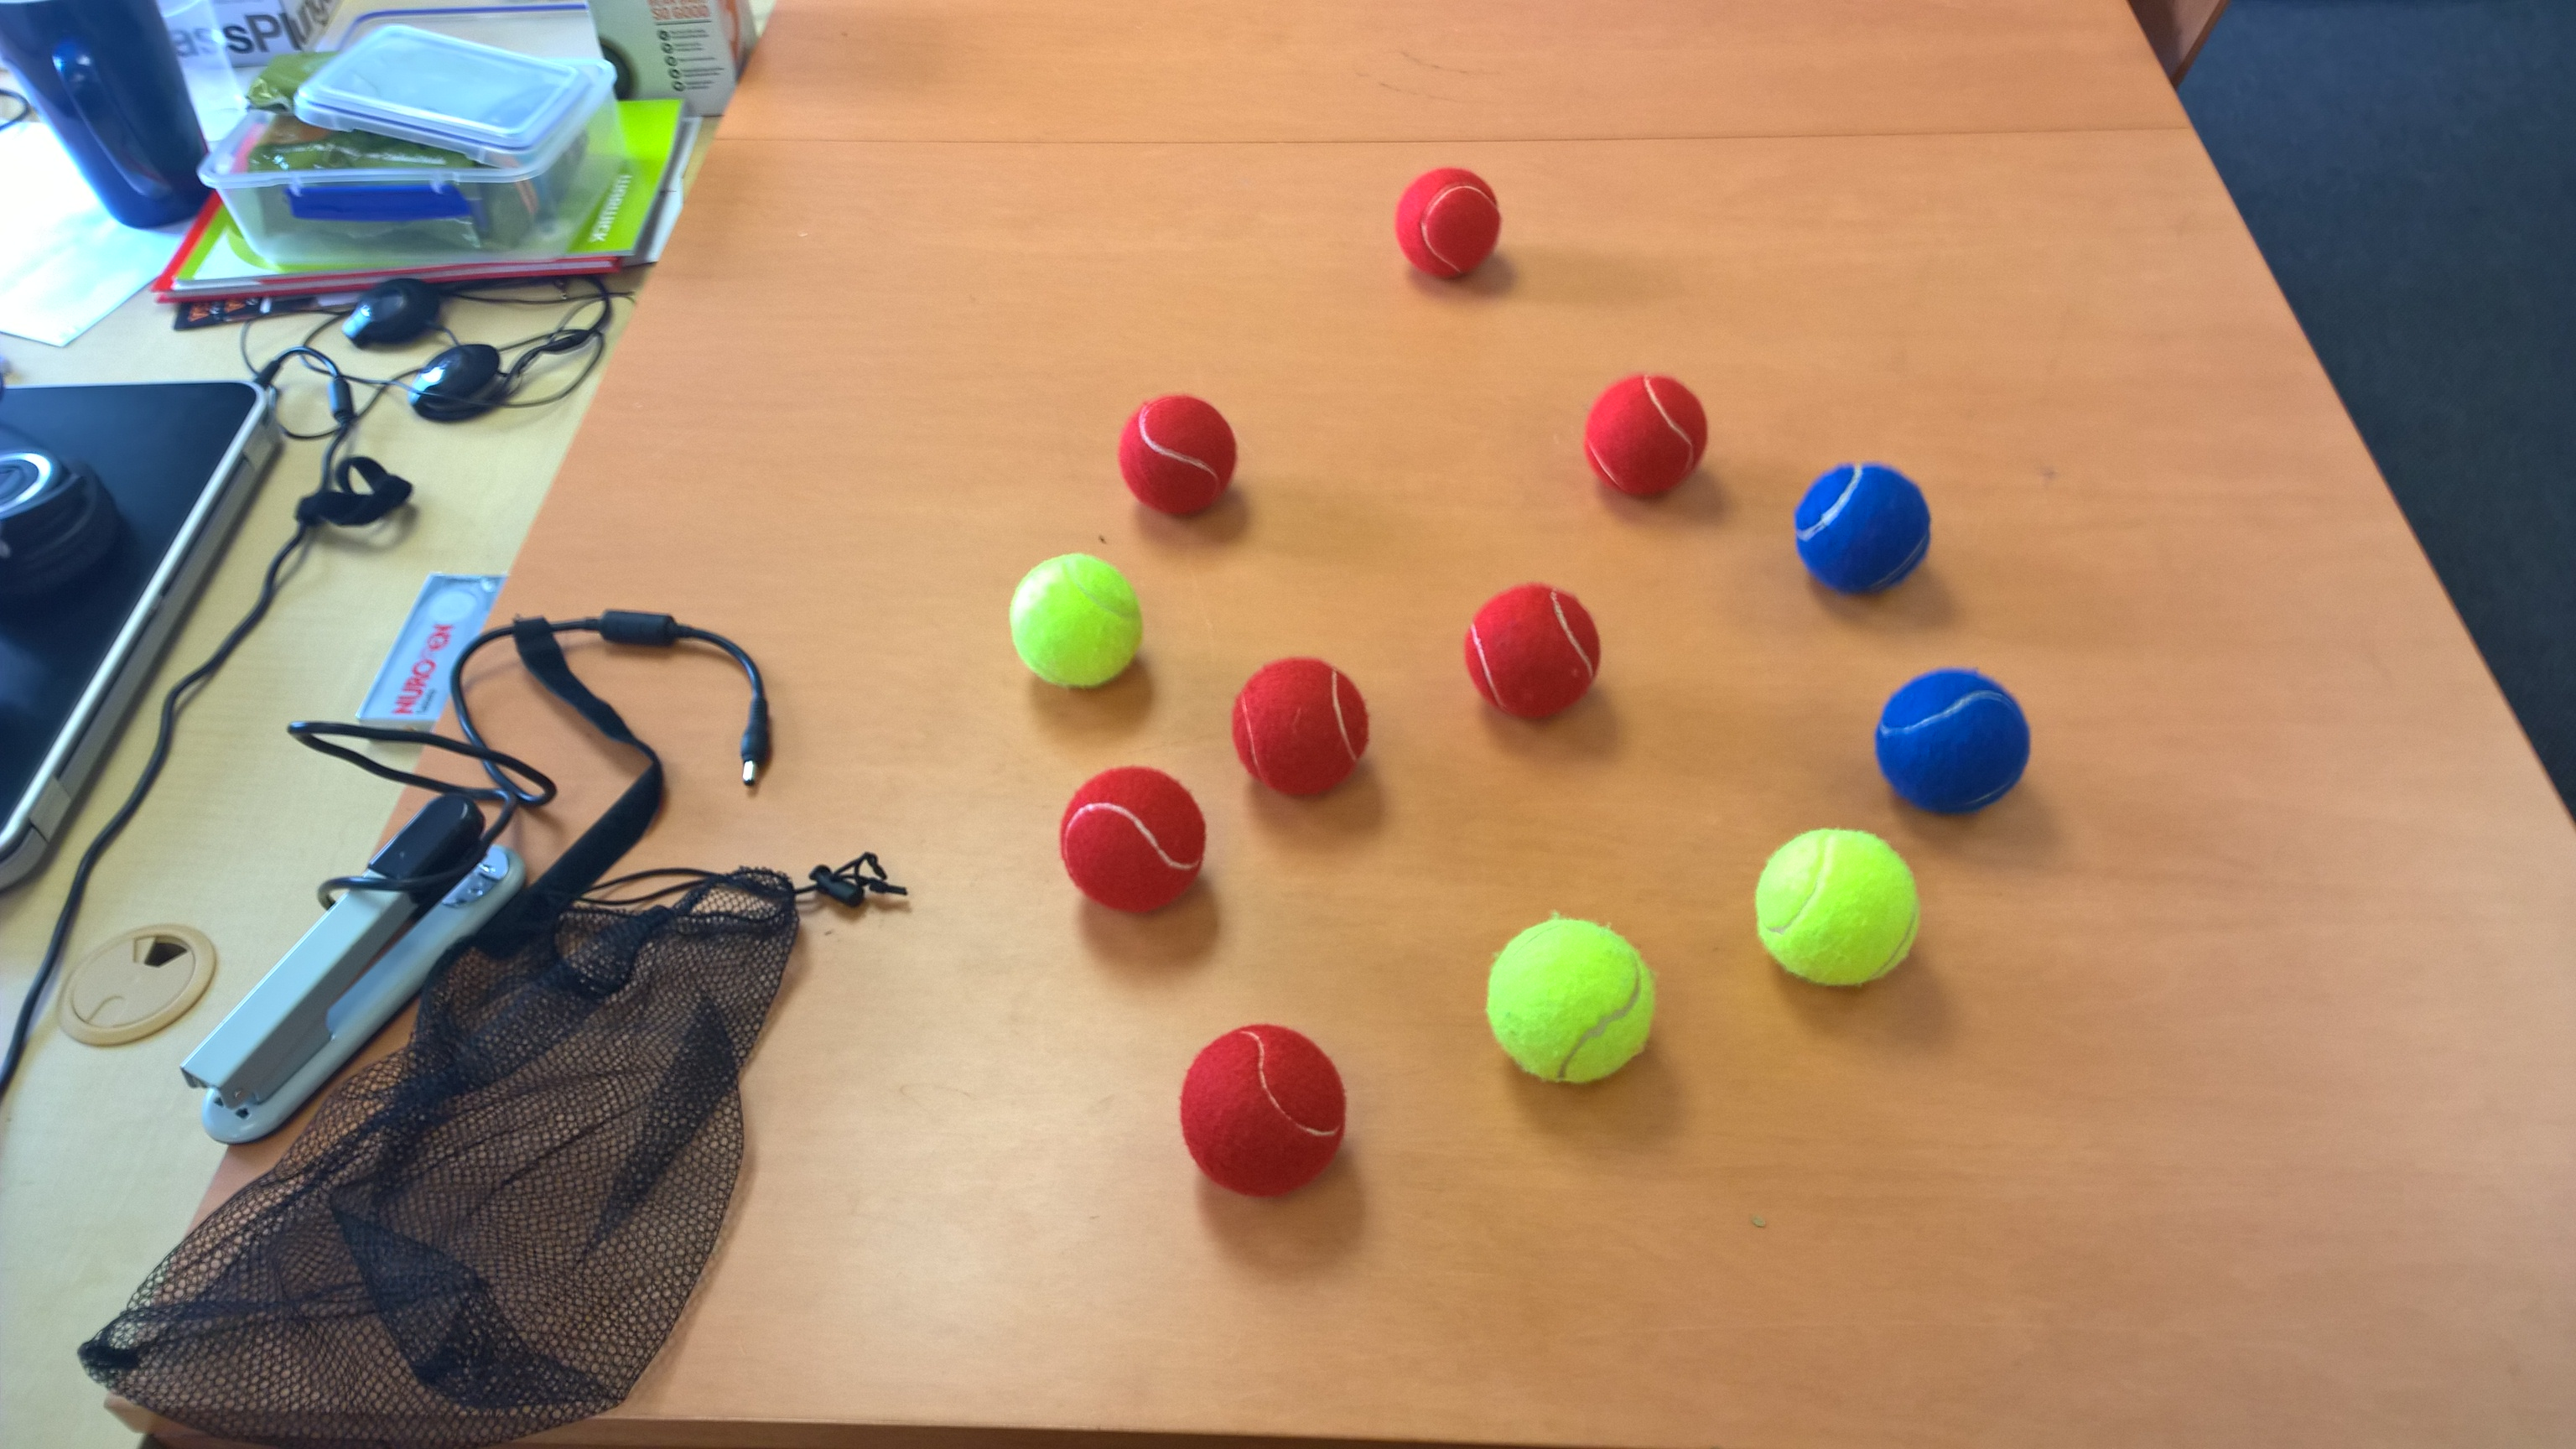
\includegraphics[width=\linewidth]{images/Image_1}
  \caption{Original Image}
  \label{fig:Original Image}
\end{figure}

A full break down of the process has been attached and can be found in the code in the appendix.

%%%%%%%%%%%%%%%%%%%%%%%%%%%%%%%%%%%%%%%%%%%%%%%%%%%%%%%%%%%%%%%%%%%%%%%%%%%%%%%%
\clearpage
\subsection{Greyscale}

Using the greyscale function to convert the image to black and white will help reduce the processing errors.

\begin{lstlisting}[language = C++]
	//Convert to greyscale
	cvtColor(image, greyscale, CV_BGR2GRAY);
	imwrite("Grey Scale.jpg", greyscale);	//Save greyscale
\end{lstlisting} 

\begin{figure}[H]
  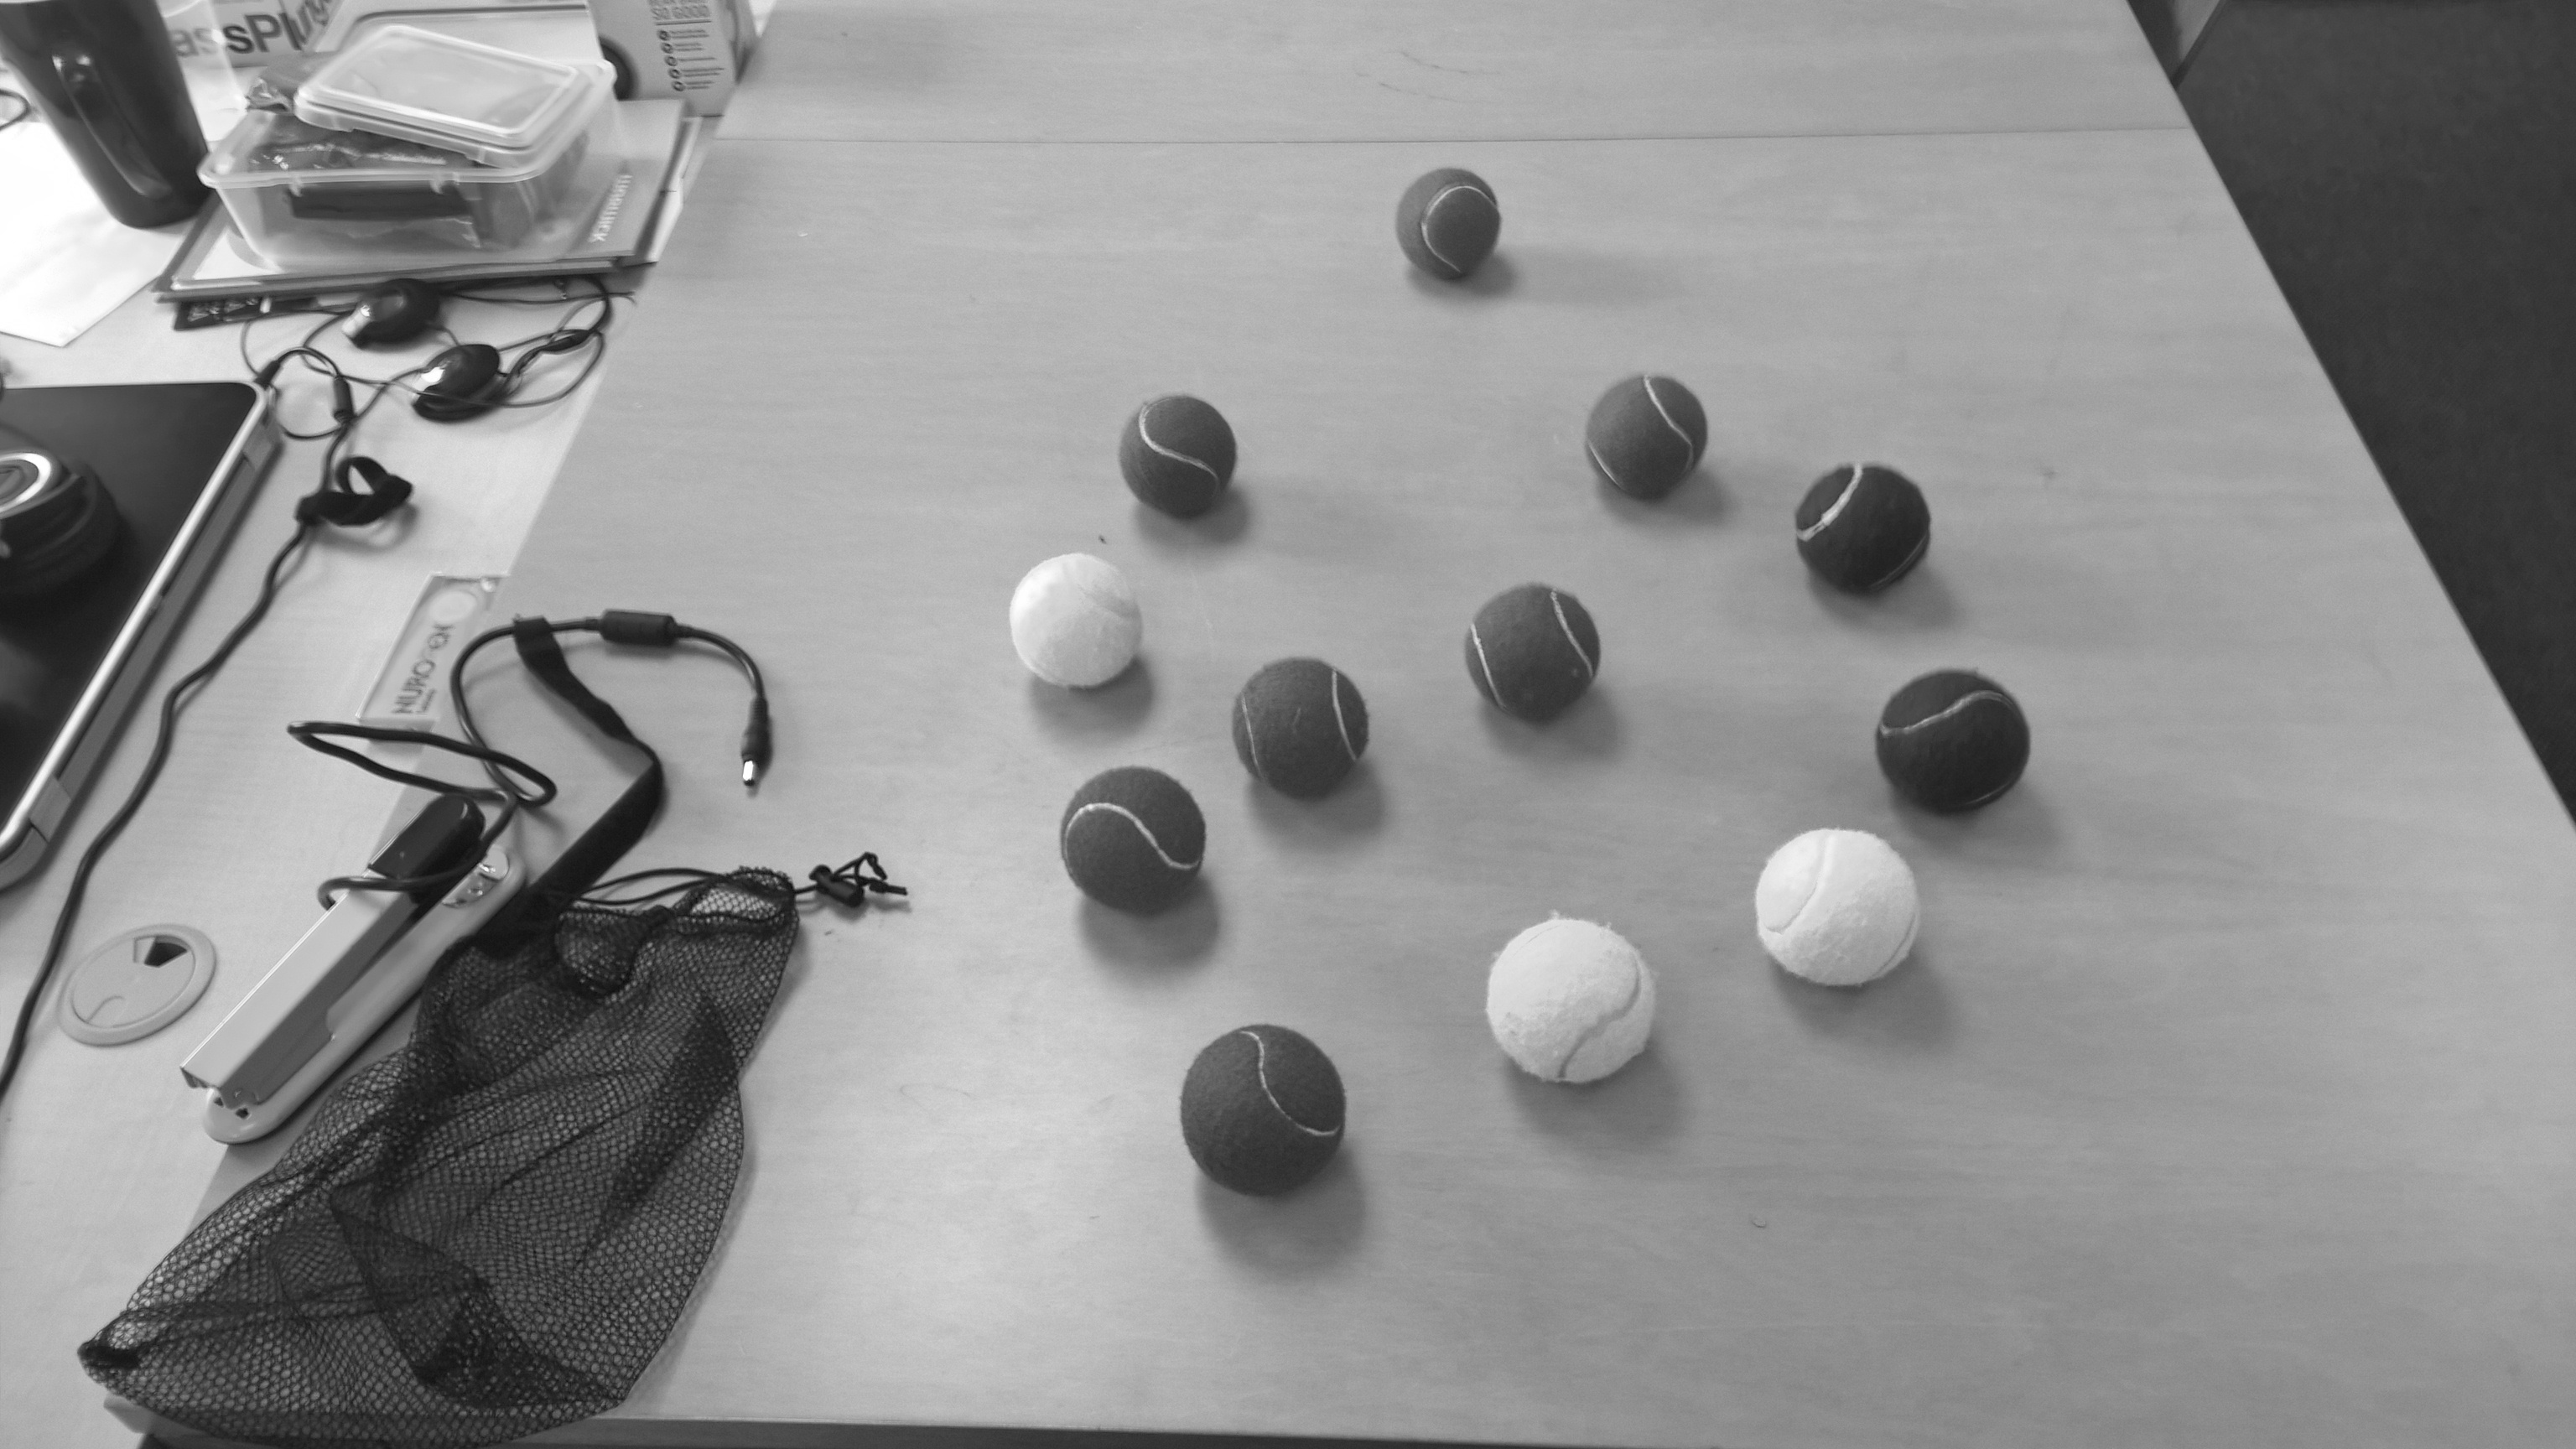
\includegraphics[width=\linewidth]{images/GreyScale}
  \caption{Greyscale filter}
  \label{fig:Greyscale filter}
\end{figure}

%%%%%%%%%%%%%%%%%%%%%%%%%%%%%%%%%%%%%%%%%%%%%%%%%%%%%%%%%%%%%%%%%%%%%%%%%%%%%%%%
\clearpage
\subsection{Gaussian Blur}

The Gaussian blur and smoothing is used to reduce the noise of the image to help eliminate any external influences. The function will transform the image using convolution matrix, and will give a result based on each pixel and it's surrounding pixels to contour and blur while maintaining the edges integerity.

From the naked eye it may be hard to recognise this from the image below and the previous observed; but if the image is enlarged you can clearly see the edges and pixels blended slightly.

\begin{lstlisting}[language = C++]
	//Noise reduction
	GaussianBlur(greyscale, blurred, Size(5, 5), 1.4);
	imwrite("Blurred.jpg", greyscale);		
\end{lstlisting}

\begin{figure}[H]
  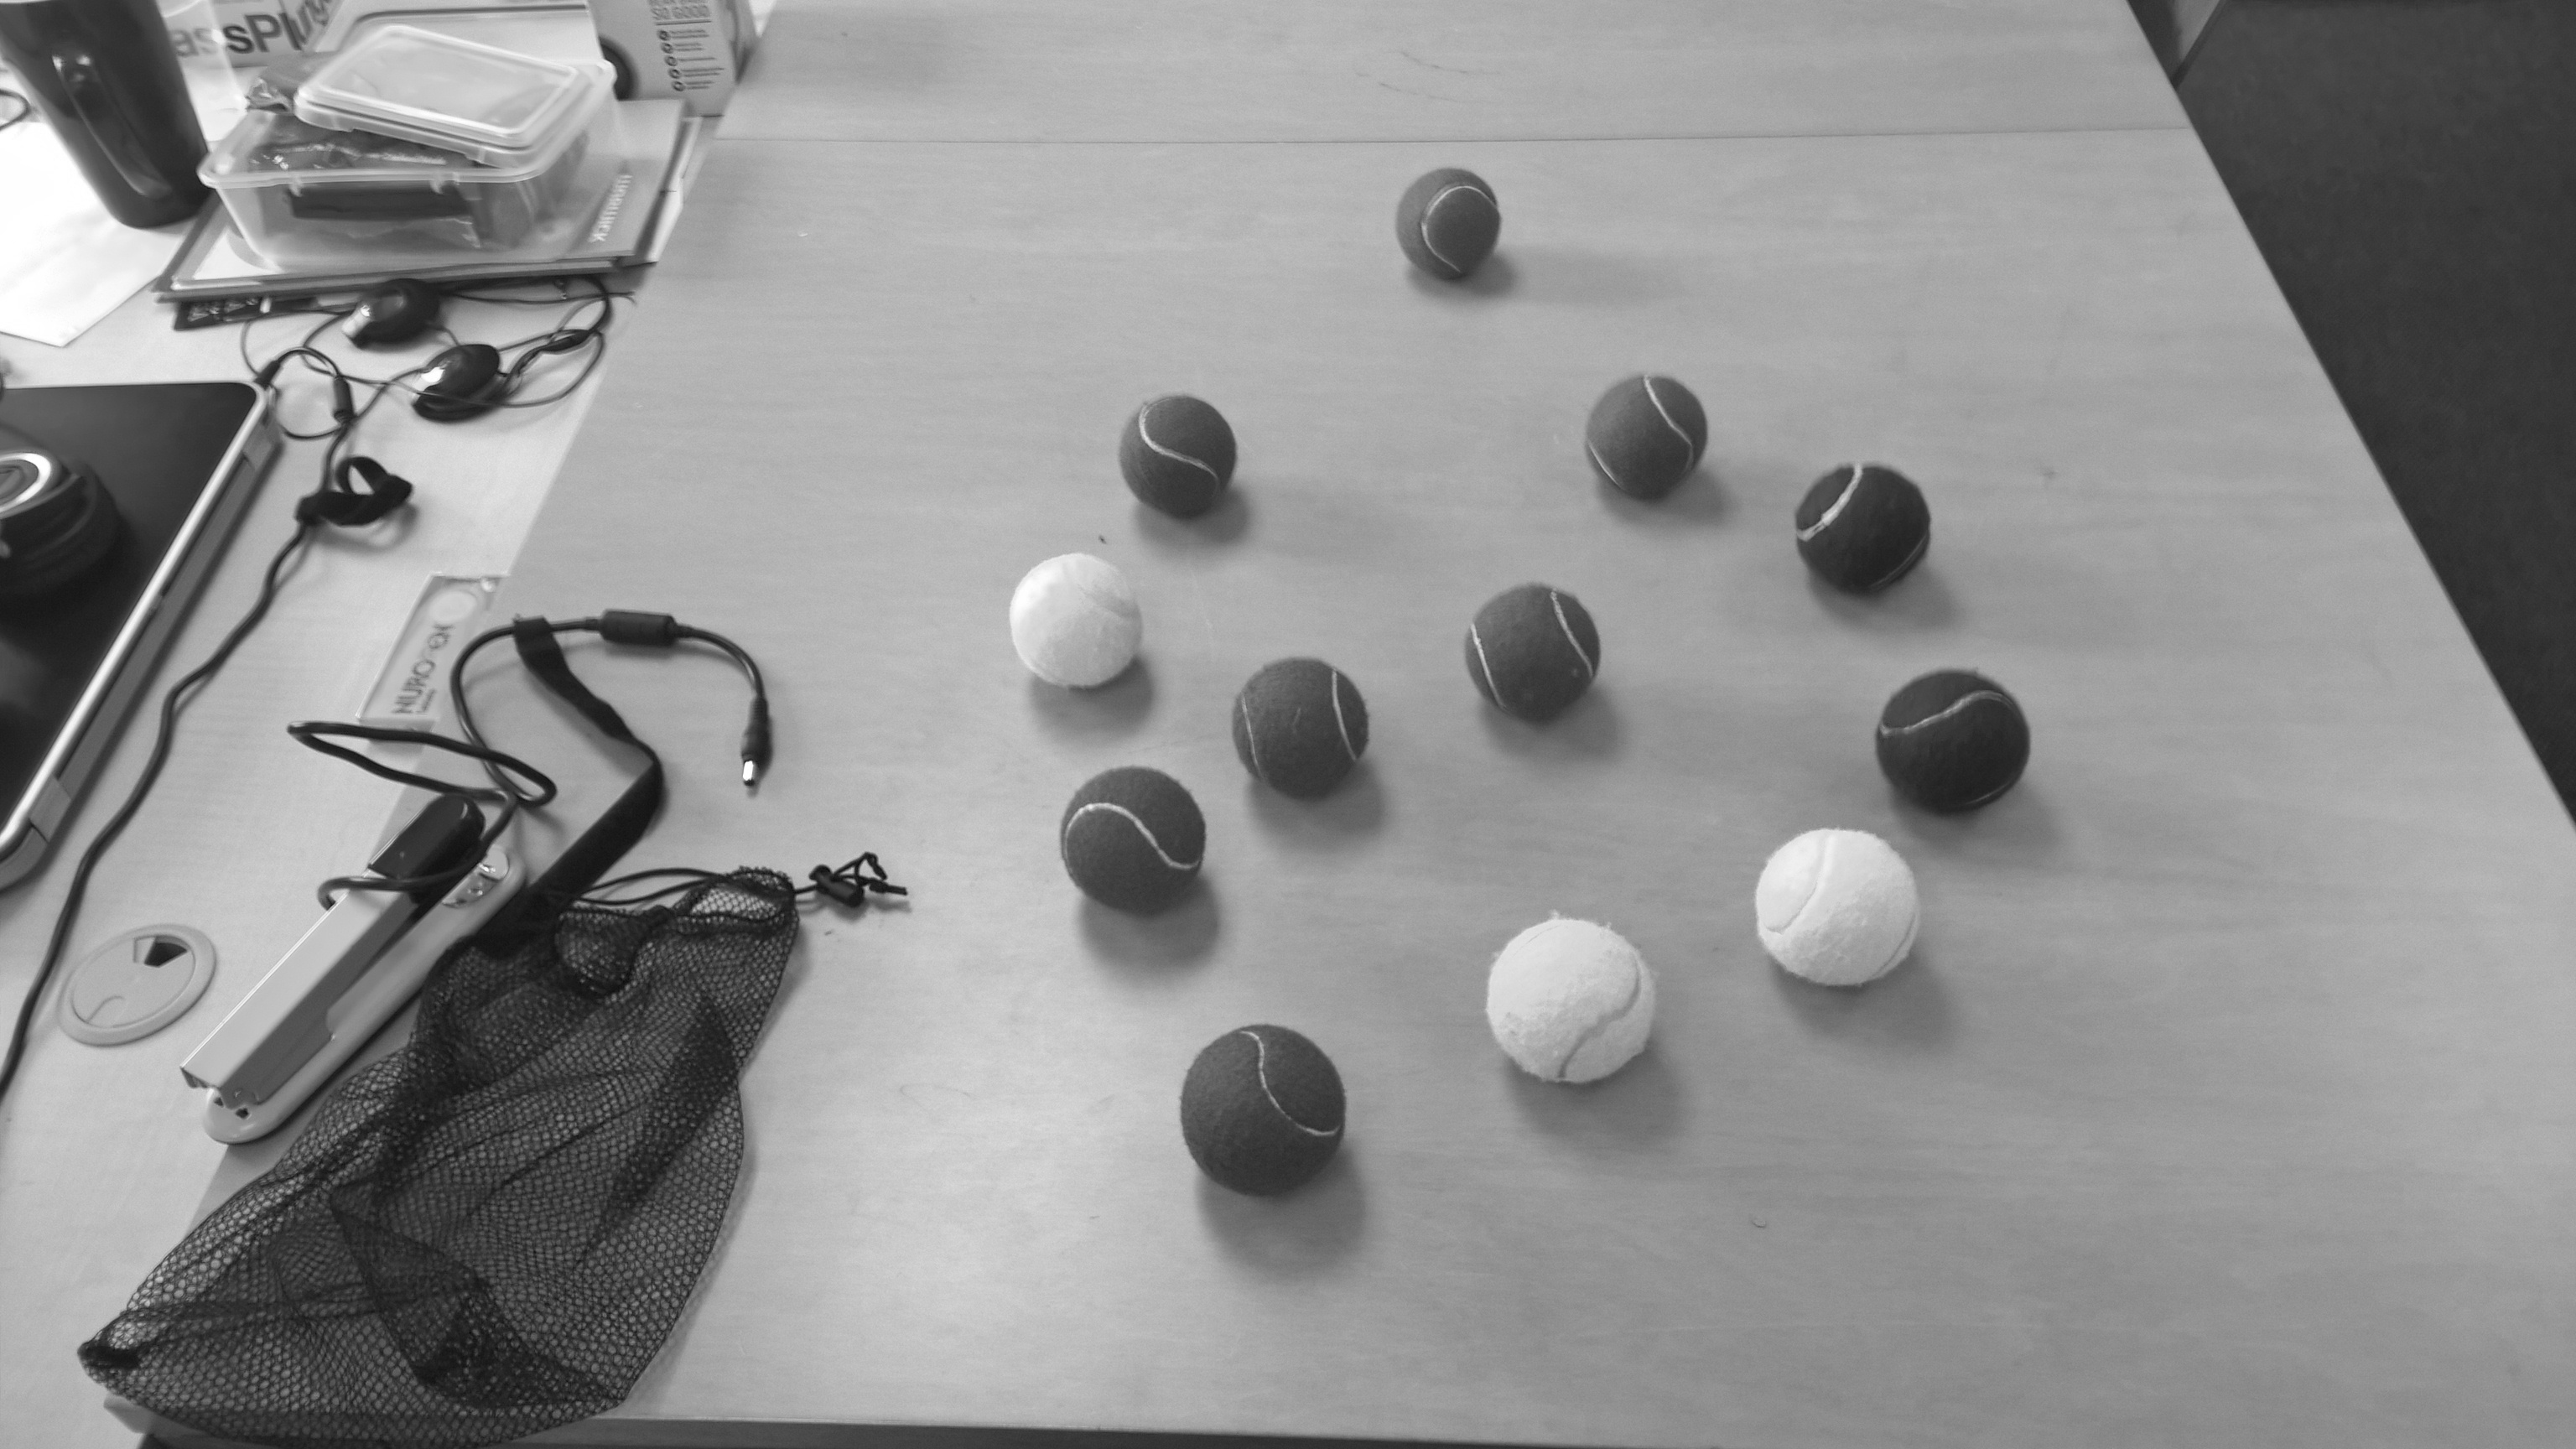
\includegraphics[width=\linewidth]{images/Blurred}
  \caption{Noise reduction with Gaussian Blur}
  \label{fig:Noise reduction with Gaussian Blur}
\end{figure}

%%%%%%%%%%%%%%%%%%%%%%%%%%%%%%%%%%%%%%%%%%%%%%%%%%%%%%%%%%%%%%%%%%%%%%%%%%%%%%%%

\subsection{Sobel operator}

The Sobel operator combines the Gaussian blur and differentiation, and is used to find an approximation of the gradient; then process and detect the edges and produce an edge map. This is a two stage process in respect to calculating two derivatives, and may only be done correctly if the original image is converted to greyscale. The result of the first step will give two outputs, each convolution gradient in the x and y directions respectfully; in the second step it will combine the two gradient direction's from the outputs in step one and produce a final output.

\begin{lstlisting}[language = C++]
	//Grad X
	Sobel(blurred, gradx, ddepth, 1, 0, 3, scale, delta, BORDER_DEFAULT);

	//Grad Y
	Sobel(blurred, grady, ddepth, 0, 1, 3, scale, delta, BORDER_DEFAULT);
\end{lstlisting}

%%%%%%%%%%%%%%%%%%%%%%%%%%%%%%%%%%%%%%%%%%%%%%%%%%%%%%%%%%%%%%%%%%%%%%%%%%%%%%%%
\clearpage
\subsection{Magnitude \& Angle}

\begin{lstlisting}[language = C++]
	//Magnitude, Angle
	cartToPolar(gradx, grady, mag, angle, true);
\end{lstlisting}

\begin{figure}[H]
  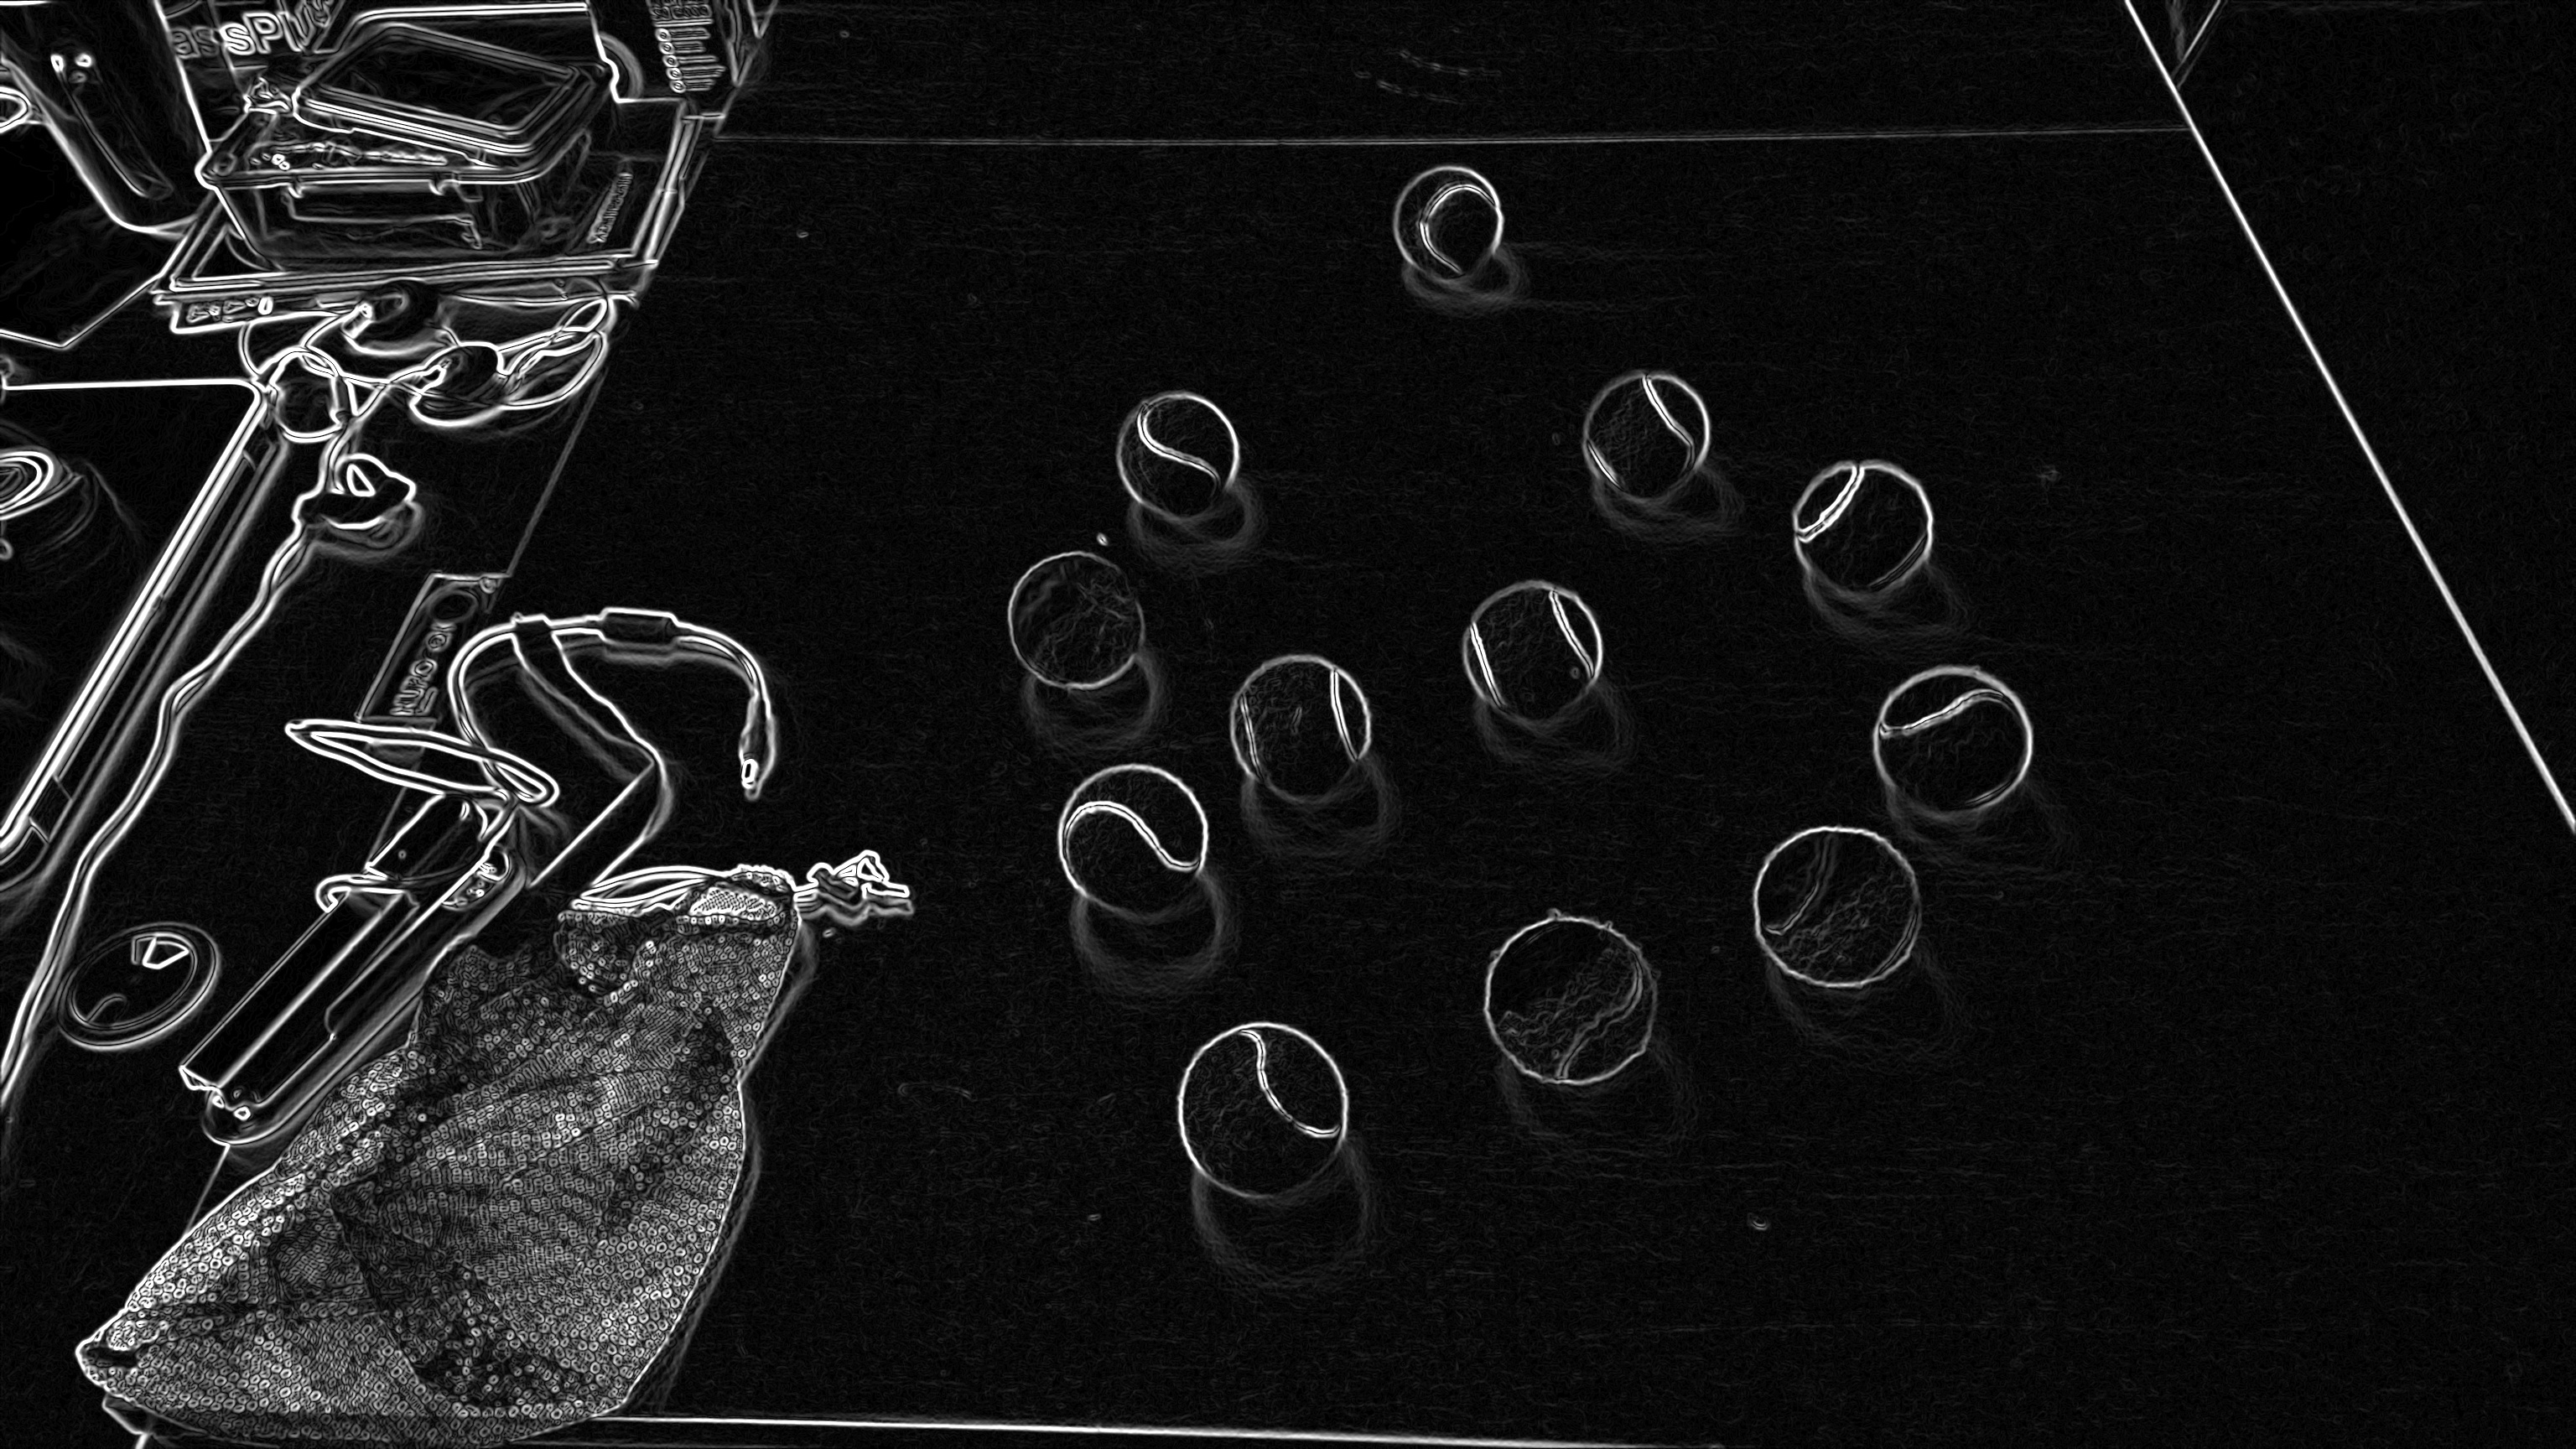
\includegraphics[width=\linewidth]{images/Mag}
  \caption{Magnitude transformations}
  \label{fig:Magnitude transformations}
\end{figure}

\begin{figure}[H]
  \includegraphics[width=\linewidth]{images/Angle}
  \caption{Angle transformations}
  \label{fig:Angle transformations}
\end{figure}


%%%%%%%%%%%%%%%%%%%%%%%%%%%%%%%%%%%%%%%%%%%%%%%%%%%%%%%%%%%%%%%%%%%%%%%%%%%%%%%%

\subsection{Non Maximum Suppression}

Going through all the pixels and and finding the surrounding pixels meeting the requirements at each point in respect to one another, then writing to that pixel if it what is found to be an edge white, or if found some requirements met write pixel grey, else non of the conditions were met and write the pixel black.

Below is a function called to find the Non Maximum Suppression render, thresholding also takes place simultaneously to this stage.

\begin{lstlisting}[language = C++]
//Non Max Suppression
Mat maxsuppress(Mat mag, Mat angle){
	Mat suppress;
	float clr;
	suppress = Mat(mag.rows, mag.cols, CV_32F);
	for (int y = 1; y < mag.rows - 1; y++) {
		for (int x = 1; x < mag.cols - 1; x++) {
			float anglem = angle.at<float>(y, x);
			if (((anglem > 337.5) && (anglem <= 0)) || ((anglem <= 22.5) && (anglem > 0)) || ((anglem > 157.5) && (anglem <= 202.5))){
				//Thresholding takes place here, code removed for reference 
				suppress.at<float>(y, x) = clr;
			}
			if (((anglem > 22.5) && (anglem <= 67.5)) || ((anglem > 202.5) && (anglem <= 247.5))){
				//Thresholding takes place here, code removed for reference 
				suppress.at<float>(y, x) = clr;
			}
			if (((anglem > 67.5) && (anglem <= 112.5)) || ((anglem > 245.5) && (anglem <= 292.5))){
				//Thresholding takes place here, code removed for reference 
				suppress.at<float>(y, x) = clr;
			}
			if (((anglem > 112.5) && (anglem <= 157.5)) || ((anglem > 292.5) && (anglem <= 337.5))){
				//Thresholding takes place here, code removed for reference 
				suppress.at<float>(y, x) = clr;
			}
		}
	}
	return suppress;
}
\end{lstlisting}


%%%%%%%%%%%%%%%%%%%%%%%%%%%%%%%%%%%%%%%%%%%%%%%%%%%%%%%%%%%%%%%%%%%%%%%%%%%%%%%%
\clearpage
\subsection{Thresholding}

Along side the Non Maximum Suppression, once a value has been found the threshold will check to see if the value is greater or lower then the set point, and in turn write the pixel white or grey; if these conditions are not met then the pixel will be made black.

\begin{lstlisting}[language = C++]
				//Thresholding
				if ((mag.at<float>(y, x - 1) < mag.at<float>(y, x)) && (mag.at<float>(y, x) > mag.at<float>(y, x + 1))){
					if (mag.at<float>(y, x) > 70) {
						clr = 255.0;
					}
					if ((mag.at<float>(y, x) < 70) && (mag.at<float>(y, x) < 1))
						clr = 100.0;
				}
				else {
					clr = 0.0;
				}
\end{lstlisting}

\begin{figure}[H]
  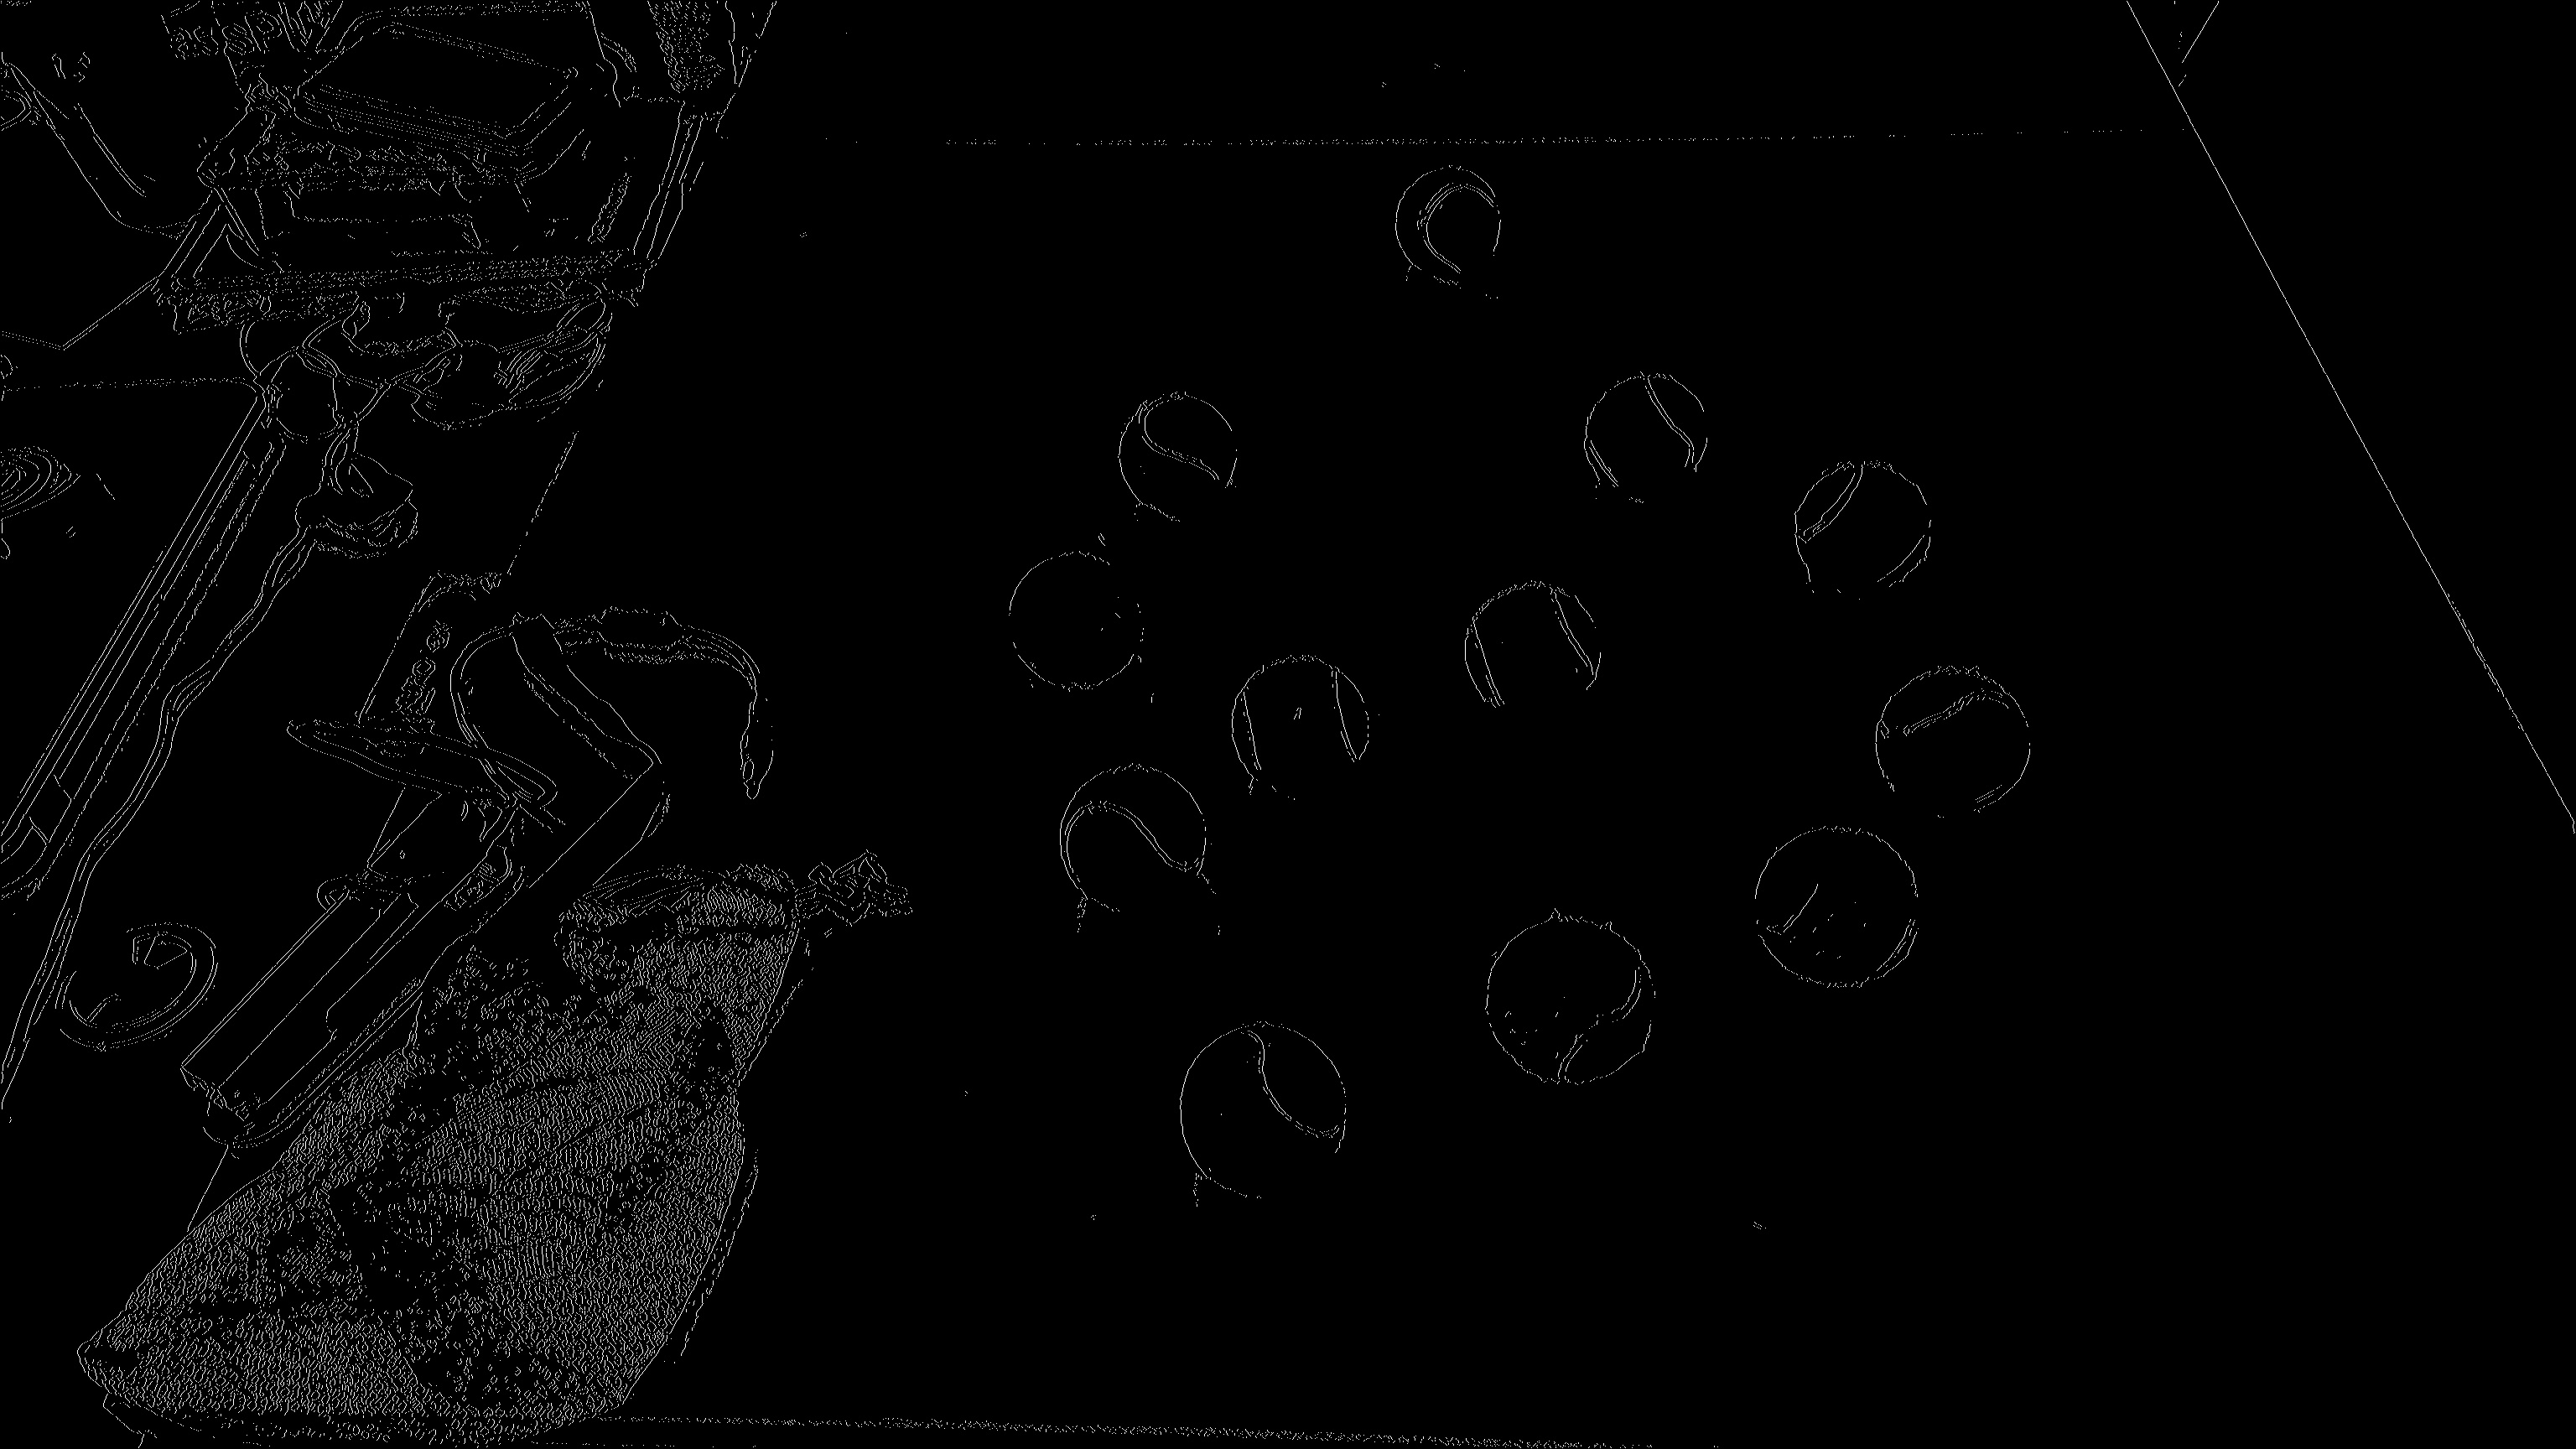
\includegraphics[width=\linewidth]{images/MaxSuppression}
  \caption{Non Maximum Suppression with Thresholding}
  \label{fig:Non Maximum Suppression with Thresholding}
\end{figure}


%%%%%%%%%%%%%%%%%%%%%%%%%%%%%%%%%%%%%%%%%%%%%%%%%%%%%%%%%%%%%%%%%%%%%%%%%%%%%%%%
\clearpage
\subsection{Hysteresis}

The Hysteresis recursive function is the called to edit the non-maximum suppression image via a pointer, and will enhance all the lines connecting the whites where possible.

\begin{lstlisting}[language = C++]
void hysterysis(int y, int x, Mat *suppress) {
	if (suppress->at<float>(y, x + 1) == 100) {
		suppress->at<float>(y, x + 1) = 255.0;
		hysterysis(y, x + 1, suppress);
	}
	if (suppress->at<float>(y, x - 1) == 100) {
		suppress->at<float>(y, x - 1) = 255.0;
		hysterysis(y, x - 1, suppress);
	}
	if (suppress->at<float>(y + 1, x) == 100) {
		suppress->at<float>(y + 1, x) = 255.0;
		hysterysis(y + 1, x, suppress);
	}
	if (suppress->at<float>(y - 1, x) == 100) {
		suppress->at<float>(y - 1, x) = 255.0;
		hysterysis(y - 1, x, suppress);
	}
	if (suppress->at<float>(y - 1, x + 1) == 100) {
		suppress->at<float>(y - 1, x + 1) = 255.0;
		hysterysis(y - 1, x + 1, suppress);
	}
	if (suppress->at<float>(y - 1, x - 1) == 100) {
		suppress->at<float>(y - 1, x - 1) = 255.0;
		hysterysis(y - 1, x - 1, suppress);
	}
	if (suppress->at<float>(y + 1, x + 1) == 100) {
		suppress->at<float>(y + 1, x + 1) = 255.0;
		hysterysis(y + 1, x + 1, suppress);
	}
	if (suppress->at<float>(y + 1, x - 1) == 100) {
		suppress->at<float>(y + 1, x - 1) = 255.0;
		hysterysis(y + 1, x - 1, suppress);
	}
	else { 
		suppress->at<float>(y,x) = 0.0;
	}
}
\end{lstlisting}

%%%%%%%%%%%%%%%%%%%%%%%%%%%%%%%%%%%%%%%%%%%%%%%%%%%%%%%%%%%%%%%%%%%%%%%%%%%%%%%%
%%%%%%%%%%%%%%%%%%%%%%%%%%%%%%%%%%%%%%%%%%%%%%%%%%%%%%%%%%%%%%%%%%%%%%%%%%%%%%%%
\clearpage

\section{RESULTS}

The final result from original image, to the final image of rendered edges only.

\begin{figure}[H]
  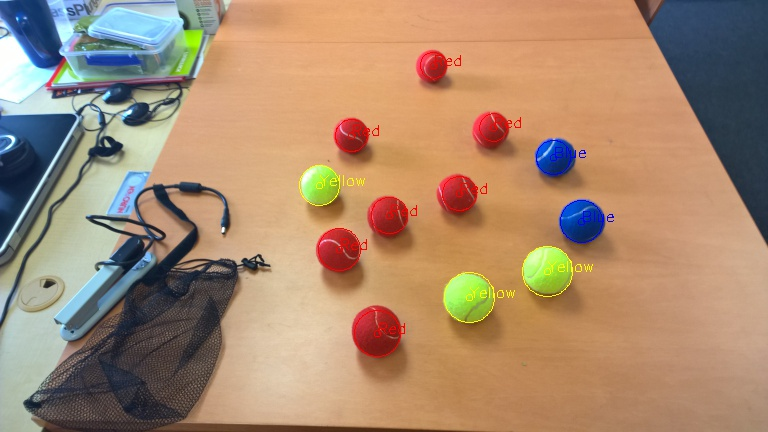
\includegraphics[width=\linewidth]{images/Final}
  \caption{The final image is given of the edges only}
  \label{fig:The final image is given of the edges only}
\end{figure}


%%%%%%%%%%%%%%%%%%%%%%%%%%%%%%%%%%%%%%%%%%%%%%%%%%%%%%%%%%%%%%%%%%%%%%%%%%%%%%%%

\subsection{Fine Tuning} 
While the process is straight forward and consists of step by step operations, the procedure in which required fine tuning. This involves checking the matrix at different points and the threshold values.

%%%%%%%%%%%%%%%%%%%%%%%%%%%%%%%%%%%%%%%%%%%%%%%%%%%%%%%%%%%%%%%%%%%%%%%%%%%%%%%%

\subsection{Testing}
Each step has an output image saved to check the processes respectively. The images are checked to make sure each stage is completing the task correctly, if not the code is then referred to and further revisions are made.


%%%%%%%%%%%%%%%%%%%%%%%%%%%%%%%%%%%%%%%%%%%%%%%%%%%%%%%%%%%%%%%%%%%%%%%%%%%%%%%%

\subsection{Finalising}
Making the program stable and concise, and as robust as possible builds for a good design. The method of testing all effects of the convolution matrix that might effect the system is required to make this achievable in getting the desired edge values. 


%%%%%%%%%%%%%%%%%%%%%%%%%%%%%%%%%%%%%%%%%%%%%%%%%%%%%%%%%%%%%%%%%%%%%%%%%%%%%%%%
%%%%%%%%%%%%%%%%%%%%%%%%%%%%%%%%%%%%%%%%%%%%%%%%%%%%%%%%%%%%%%%%%%%%%%%%%%%%%%%%
\clearpage
\section{CONCLUSIONS}

The final image detection and edge render has been produced from several steps; this method while not exact is a basic idea of how the Canny operator works. The steps taken were to use the OpenCV functions to greyscale the image, then take that converted colour and run it through Gaussian blurring to reduce noise. After the transformation and noise reduction the Sobel operator is called to determine the gradients, and then cartToPolar function is used to convert these gradients to magnitudes and angles. The Non Suppression filter is then implemented with a threshold to produce more stable lines for the edges; and finally the Hysteresis stage is called to reduce the noise and threshold function to get rid of any grey static left over.

The result of the described method has been found similar to that of the canny detection method and the edges, while not perfectly shown are in the correct areas.

%%%%%%%%%%%%%%%%%%%%%%%%%%%%%%%%%%%%%%%%%%%%%%%%%%%%%%%%%%%%%%%%%%%%%%%%%%%%%%%%
%%%%%%%%%%%%%%%%%%%%%%%%%%%%%%%%%%%%%%%%%%%%%%%%%%%%%%%%%%%%%%%%%%%%%%%%%%%%%%%%

\nocite{*}
\bibliographystyle{ieeetr}
\bibliography{references}

%%%%%%%%%%%%%%%%%%%%%%%%%%%%%%%%%%%%%%%%%%%%%%%%%%%%%%%%%%%%%%%%%%%%%%%%%%%%%%%%
%%%%%%%%%%%%%%%%%%%%%%%%%%%%%%%%%%%%%%%%%%%%%%%%%%%%%%%%%%%%%%%%%%%%%%%%%%%%%%%%

\clearpage
\section*{APPENDIX}

\begin{lstlisting}[language = C++]
#include <opencv2\opencv.hpp>
#include <opencv2/core.hpp>
#include <opencv2/imgcodecs.hpp>
#include <opencv2/highgui.hpp>

#include <iostream>
#include <string>

using namespace cv;
using namespace std;

Mat maxsuppress(Mat mag, Mat angle);
void hysterysis(int y, int x, Mat *suppress);

int main(int, char** argv){

	Mat image, greyscale, blurred, maxsuppression, finalimage;
	
	//Read in the image
	image = imread("Image 1.jpg", IMREAD_COLOR);   

	//Convert to greyscale
	cvtColor(image, greyscale, CV_BGR2GRAY);
	imwrite("Grey Scale.jpg", greyscale);	//Save greyscale

	//Noise reduction
	GaussianBlur(greyscale, blurred, Size(5, 5), 1.4);
	imwrite("Blurred.jpg", greyscale);		//Save blurred

	//Gradient
	Mat gradx, grady, mag, angle;
	int scale = 2, delta = 0, ddepth = CV_32F;

	//Grad X
	Sobel(blurred, gradx, ddepth, 1, 0, 3, scale, delta, BORDER_DEFAULT);

	//Grad Y
	Sobel(blurred, grady, ddepth, 0, 1, 3, scale, delta, BORDER_DEFAULT);

	//Magnitude, Angle
	cartToPolar(gradx, grady, mag, angle, true);

	//Save images
	imwrite("Mag.jpg", mag);
	imwrite("Angle.jpg", angle);

	maxsuppression = maxsuppress(mag, angle);
	imwrite("MaxSuppression.jpg", maxsuppression);

	for (int y = 1; y < mag.rows - 1; y++) {
		for (int x = 1; x < mag.cols - 1; x++) {
			if (mag.at<float>(y, x) == 255.0) {
				hysterysis(mag.rows, mag.cols, &maxsuppression);
			}
		}
	}

	threshold(maxsuppression, maxsuppression, 245, 255, 0);
	
	imwrite("Final.jpg", maxsuppression);

	waitKey(27);
	destroyAllWindows();
	return 0;
}

//Non Max Suppression
Mat maxsuppress(Mat mag, Mat angle){
	Mat suppress;
	float clr;
	suppress = Mat(mag.rows, mag.cols, CV_32F);
	for (int y = 1; y < mag.rows - 1; y++) {
		for (int x = 1; x < mag.cols - 1; x++) {
			float anglem = angle.at<float>(y, x);
			if (((anglem > 337.5) && (anglem <= 0)) || ((anglem <= 22.5) && (anglem > 0)) || ((anglem > 157.5) && (anglem <= 202.5))){
				//Thresholding
				if ((mag.at<float>(y, x - 1) < mag.at<float>(y, x)) && (mag.at<float>(y, x) > mag.at<float>(y, x + 1))){
					if (mag.at<float>(y, x) > 70) {
						clr = 255.0;
					}
					if ((mag.at<float>(y, x) < 70) && (mag.at<float>(y, x) < 1))
						clr = 100.0;
				}
				else {
					clr = 0.0;
				}
				suppress.at<float>(y, x) = clr;
			}
			if (((anglem > 22.5) && (anglem <= 67.5)) || ((anglem > 202.5) && (anglem <= 247.5))){
				//Thresholding
				if ((mag.at<float>(y, x - 1) < mag.at<float>(y, x)) && (mag.at<float>(y, x) > mag.at<float>(y, x + 1))){
					if (mag.at<float>(y, x) > 70) {
						clr = 255.0;
					}
					if ((mag.at<float>(y, x) < 70) && (mag.at<float>(y, x) < 1))
						clr = 100.0;
				}
				else {
					clr = 0.0;
				}
				suppress.at<float>(y, x) = clr;
			}
			if (((anglem > 67.5) && (anglem <= 112.5)) || ((anglem > 245.5) && (anglem <= 292.5))){
				//Thresholding
				if ((mag.at<float>(y, x - 1) < mag.at<float>(y, x)) && (mag.at<float>(y, x) > mag.at<float>(y, x + 1))){
					if (mag.at<float>(y, x) > 70) {
						clr = 255.0;
					}
					if ((mag.at<float>(y, x) < 70) && (mag.at<float>(y, x) < 1))
						clr = 100.0;
				}
				else {
					clr = 0.0;
				}
				suppress.at<float>(y, x) = clr;
			}
			if (((anglem > 112.5) && (anglem <= 157.5)) || ((anglem > 292.5) && (anglem <= 337.5))){
				//Thresholding
				if ((mag.at<float>(y, x - 1) < mag.at<float>(y, x)) && (mag.at<float>(y, x) > mag.at<float>(y, x + 1))){
					if (mag.at<float>(y, x) > 70) {
						clr = 255.0;
					}
					if ((mag.at<float>(y, x) < 70) && (mag.at<float>(y, x) < 1))
						clr = 100.0;
				}
				else {
					clr = 0.0;
				}
				suppress.at<float>(y, x) = clr;
			}
		}
	}
	return suppress;
}

void hysterysis(int y, int x, Mat *suppress) {
	if (suppress->at<float>(y, x + 1) == 100) {
		suppress->at<float>(y, x + 1) = 255.0;
		hysterysis(y, x + 1, suppress);
	}
	if (suppress->at<float>(y, x - 1) == 100) {
		suppress->at<float>(y, x - 1) = 255.0;
		hysterysis(y, x - 1, suppress);
	}
	if (suppress->at<float>(y + 1, x) == 100) {
		suppress->at<float>(y + 1, x) = 255.0;
		hysterysis(y + 1, x, suppress);
	}
	if (suppress->at<float>(y - 1, x) == 100) {
		suppress->at<float>(y - 1, x) = 255.0;
		hysterysis(y - 1, x, suppress);
	}
	if (suppress->at<float>(y - 1, x + 1) == 100) {
		suppress->at<float>(y - 1, x + 1) = 255.0;
		hysterysis(y - 1, x + 1, suppress);
	}
	if (suppress->at<float>(y - 1, x - 1) == 100) {
		suppress->at<float>(y - 1, x - 1) = 255.0;
		hysterysis(y - 1, x - 1, suppress);
	}
	if (suppress->at<float>(y + 1, x + 1) == 100) {
		suppress->at<float>(y + 1, x + 1) = 255.0;
		hysterysis(y + 1, x + 1, suppress);
	}
	if (suppress->at<float>(y + 1, x - 1) == 100) {
		suppress->at<float>(y + 1, x - 1) = 255.0;
		hysterysis(y + 1, x - 1, suppress);
	}
	else { 
		suppress->at<float>(y,x) = 0.0;
	}
}

\end{lstlisting}

\end{document}
